\chapter{Fundamentação Teórica} \label{fundamentacao}
Neste capitulo será discutido as teorias que embasam a compatibilidade eletromagnética, quais as problematizações que são inerentes em análises de compatibilidade eletromagnética, as formas como estas são realizadas. Especificamente será abordado o estudo da compatibilidade eletromagnética em PCIs. %, quais medidas são realizadas e que tipos de técnicas se encontram no estado da arte nesta realização.

\section{Compatibilidade Eletromagnética}
% Aspectos Gerais da EMC
Desde o advento das comunicações telegráficas e do rádio até os dias atuais com sistemas muito mais complexos de comunicação (radares, estações de rádio, TV, telefonia móvel, satélites), e, cada vez mais sendo utilizados sistemas eletrônicos (dispositivos, equipamentos, etc...) a interferência eletromagnética é tema de interesse e estudo de cientistas e engenheiros das áreas de comunicações e eletricidade~\cite[p.~1]{paul2006}.

Segundo~\citeonline[p.~3]{paul2006} o estudo da Compatibilidade Eletromagnética (EMC) se concentra em investigar três aspectos fundamentais: \textit{Geração, Transmissão e Recepção} de sinais eletromagnéticos. A interação dos sinais gerados no transmissor com o receptor pode interferir no receptor ou até mesmo em si próprio (transmissor), esta interferência pode gerar uma não compatibilidade eletromagnética (porém isso não necessariamente é sempre válido) quando esta interferência acarreta em mal funcionamento em si próprio (transmissor) ou no receptor (ou em demais equipamentos eletrônicos) é necessário uma correção na exata fonte do sinal indesejado, para isso são necessários métodos de investigações afim de identificar com precisão esta fonte. O tipo de transmissão que leva a esta \textit{interferência} define o tipo de acoplamento, ou por meios de sinais eletromagnéticos conduzidos, ou por meios de sinais eletromagnéticos irradiados.

Na figura~\ref{fig:EMC_couplling_problem} ~\citeonline[p.~3]{paul2006} traz de forma sintética esses três principais aspectos no estudo da compatibilidade eletromagnética, a fonte ou emissor (\textit{source}) produz a emissão que é transmitida através do acoplamento (meio pelo qual a emissão é acoplada, ou de forma conduzida ou irradiada) até o receptor.

\begin{figure}[htb!]
	\centering 
	\caption{Aspecto Geral do Estudo de EMC}
	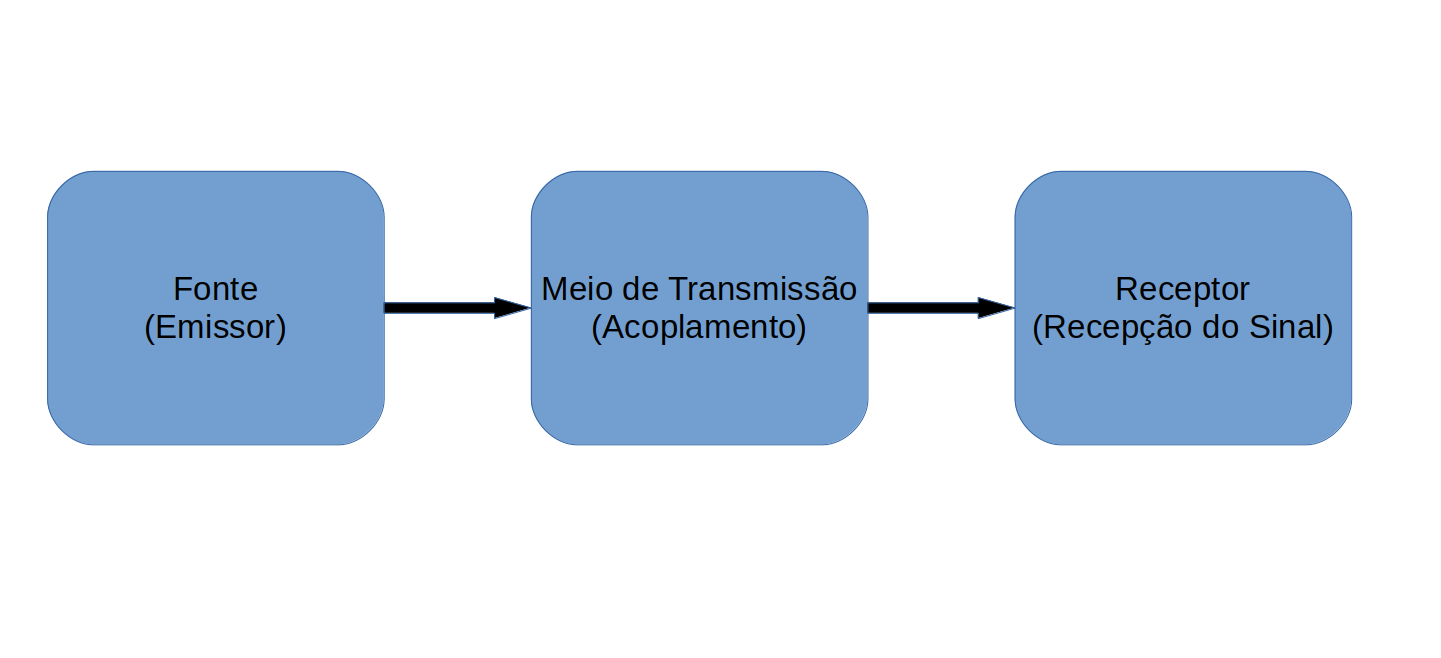
\includegraphics[scale=0.4]{./img/fundamentacao_001}
	\fonte{Adaptado de ~\citeonline[p.~3]{paul2006}}
	%\legend{\hspace{-218pt}Fonte:~\citeonline[p.~3]{paul2006}}
	\label{fig:EMC_couplling_problem}
\end{figure}

Uma das principais preocupações do estudo da EMC está em atender as normas legais e requisitos impostos pelas agências reguladoras, entretanto há também vários outros aspectos importantes a serem explorados pelo estudo de EMC. Na figura~\ref{fig:EMC_preocups} ~\citeonline[p.~8]{paul2006} traz alguns outros problemas importantes a serem investigados pelo estudo de EMC, podemos observar na figura~\ref{fig:EMC_preocups}(a) um problema de susceptibilidade muito comum nos dias atuais que é o da descarga eletrostática (\textit{Electrostatic Discharge} - ESD), onde o indivíduo se carrega eletrostaticamente e libera esta carga através do contato com equipamentos eletrônicos, podendo ocasionar assim mal funcionamento, deformidades ou até a destruição permanente do equipamento eletrônico, principalmente em sistemas ou equipamentos eletrônicos que utilizam Circuito Integrados (CI's). 

\begin{figure}[htb!]
	\centering 
	\caption{Outras Preocupações em EMC}
	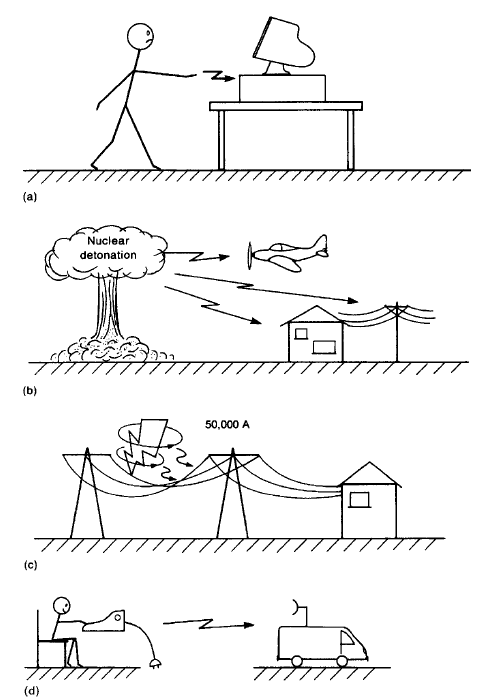
\includegraphics[scale=0.75]{./img/fundamentacao_002}
	\fonte{~\citeonline[p.~8]{paul2006}}
	%\legend{\hspace{-218pt}Fonte:~\citeonline[p.~8]{paul2006}}
	\label{fig:EMC_preocups}
\end{figure}

Ainda na figura~\ref{fig:EMC_preocups} o autor \cite[p.~8]{paul2006} traz demais preocupações do estudo de EMC, como exposto em (b) o efeito de radiações nucleares e dos pulsos eletromagnéticos (EMP) em sistemas eletrônicos embarcados, como de aviação, satélites (radiações espaciais). Em (c) temos os possíveis efeitos causados por tempestades de raios que provocam correntes na ordem $50000 A$ ocasionando campos eletromagnéticos de alta intensidade, podendo assim gerar Interferências Eletromagnéticas (EMI) em equipamentos e sistemas eletrônicos. Por fim em (d) temos a interceptação eletromagnética não autorizada, sendo a área militar e de comunicações possuidoras do maior interesse tanto na prevenção quanto na implementação.

% Historia Rápida da EMC
\subsection{Evolução temporal da EMC}
Muito provavelmente a EMI e sua correção surgiu como algo de interesse com os experimentos de Marconi no final do séc XIX~\cite[p.~10]{paul2006}. Porém, somente a partir do séc XX, na década de 1920, é que começaram a surgir artigos científicos que tratavam da EMI em rádios, tanto nos transmissores quanto nos receptores.

Durante a II Guerra Mundial, o uso de equipamentos eletrônicos, principalmente rádios, dispositivos de navegação, radares e aceleradores, ocasionou um aumento significativo por correções afim de eliminar as EMI principalmente entre rádios e aviões. Entretanto, o crescimento mais significativo das EMI ocorreu a partir do advento do transistor, na década de 1950, do Circuito Integrado (CI), na década de 1960 e do microprocessador, na década de 1970. O espectro de frequência também foi afetado, com uma maior demanda e utilização, após o crescimento da demanda por transmissão de voz e dados, isto começou a exigir maiores esforços no planejamento e regulação da utilização do espectro, o que continua até nos dias atuais ~\cite[p.~10]{paul2006}.

% Requisitos Governamentais
% Falar das Normas
Talvez o principal evento que trouxe a EMC ao nível atual de ênfase, foi a introdução do processamento digital de sinais e computação que no inicio da década de 1960 utilizavam as válvulas à vácuo, porém poucos anos mais tarde, estas foram substituídas por transistores e CI's. Com a inserção da eletrônica de estado sólido no processamento digital de sinais e computação, aumentou-se a velocidade de processamento (chaveamento) e a miniaturização dos componentes ocasionando uma aumento do espectro de frequências utilizável e uma densidade maior de \textit{ruídos} e EMI. Devido ao aumento de novos ruídos e EMI, tanto através do modo conduzido como do irradiado a \textit{Federal Communications Commision} (FCC) publicou em 1979, nos Estados Unidos, uma regulamentação para a emissão eletromagnética em todos os dispositivos digitais até certos limites. A principal intenção dessa regulamentação era trazer limites a "\textit{poluição eletromagnética}". Todavia, na Europa, já haveria ocorrido ações similares, precedentes à FCC. Já em 1933 a \textit{International Electrotechnical Commission} (IEC), em Paris na França, recomendou a criação da \textit{Comité International Special des Perturbations Radioélectriques} (CISPR). ~\citeonline[p.~11]{paul2006} salienta que "A CISPR voltou a se reunir após a Segunda Guerra Mundial em Londres em 1946. Reuniões subsequentes renderam várias publicações científicas, que abordavam com técnicas de medição, bem como limites de emissão recomendados. Alguns países europeus adotaram versões de limites recomendados pela CISPR." Sendo assim, a CISPR e a FCC se tornaram desde então as maiores precursoras de regulamentações e regras no que tange a EMI em nível global.

As regulamentações tanto da FCC quanto da CISPR tornaram a EMC uma aspecto importante para a comercialização de equipamentos e sistemas eletrônicos, visto que se estes não estiveram em conformidade com essas regulações, não poderão ser comercializados nos países que as adotam, mesmo levando-se em conta que o produto realiza sua tarefa e os clientes não se importam se o produto cumpre ou não a regulamentação estabelecida. Dessa forma, as regulamentações estatais tornaram a EMC um aspecto de suma importância no desenvolvimento de produtos e sistemas eletrônicos \cite[p.~12]{paul2006}.

\subsection{Requisitos de EMC em sistemas eletrônicos}
% Requisitos de funcionamentos de sistemas Eletrônicos 2.1(paul2006)
Basicamente há duas classes de requisitos a serem observadas no desenvolvimento de produtos/sistemas eletrônicos afim de atender a EMC, sendo estes ~\cite[p.~49]{paul2006}:

\begin{itemize}
 \item Requisitos Governamentais, Normas e Leis
 \item Requisitos Funcionais, Susceptibilidades e EMI
\end{itemize}

% Requisitos Governamentais (FCC e CISPR) 2.1(paul2006)
Devido ao estágio atual de globalização é de suma importância para os fabricantes e desenvolvedores de produtos eletrônicos estarem atentos as normas e regulamentações, tando da FCC quanto da CISPR. Nos Estados Unidos é adotado as normas da FCC~\cite{fcc47} que estabelece regulações para o rádio e comunicações cabeadas. A FCC estabelece que qualquer equipamento capaz de emitir energia, tanto por radiação quanto conduzida, estando entre $9kHz$ até $3000 GHz$ é um equipamento de rádio-frequência sujeito assim ao capitulo 15 da 47CFR ~\apud[p.~50]{fcc47}{paul2006}, na FCC ainda está definido o que é dispositivo digital:

\begin{citacao}[english]
Any unintentional radiator (device or system) that generates and uses timing pulses at a
rate in excess of 9000 pulses (cycles) per second and uses digital techniques \apud[p.~51]{fcc47}{paul2006}.
\end{citacao}

Ou seja, qualquer equipamento ou sistema de rádio-frequência que gerar ou usar pulsos de tempo que sejam superiores a $9kHz$ e que usa técnicas digitais é considerado pela FCC como um dispositivo digital. Esta definição é importante pois a FCC classifica esses produtos em duas classes: \textbf{Classe A}: São aqueles fabricados para uso comercial, industrial ou destinado a negócios; \textbf{Classe B}: são aqueles fabricados para o uso residencial ~\cite[p.~51]{paul2006}, computadores pessoais e seus periféricos são uma subcategoria de dispositivos digitais de Classe B. Os limites de emissão eletromagnética estabelcidos à Classe B são mais rigorosos do que os limites da Classe A pois supõe-se que a interferência de dispositivos em um ambiente industrial pode ser corrigida mais facilmente do que em um ambiente residencial, onde a fonte de interferência e o dispositivo susceptível estão mais próximos. Esta classificação também é adotada pela CISPR.

% EMC Conduzida e Irradiada
A FCC possui regras que estabelecem limities máximos permitidos às emissões conduzidas e irradiadas do produto digital. Emissões conduzidas são aquelas trasmitidas através de um meio condutor, um cabo, uma trilha de circuito eletrônico, etc. A faixa de freqüência para emissões conduzidas se estende de $150 kHz$ a $30 MHz$. As irradiadas são aqueles cujo o meio de transmissão é o ar ou o vácuo, ou seja, através de radiações eletromagnéticas e a faixa de frequência estabelecida pela FCC para esse tipo de emissão é de $30 MHz$ a $40 GHz$. As mesmas faixas são adotadas também pela CISPR.

A conformidade dos circuitos eletrônicos é verificada, no caso das emissões conduzidas, inserindo-se uma rede estabilizada de impedância de linha (\textit{Line Impedance Stabilization Network} - LISN) no cabo de alimentação em corrente alternada (CA) da unidade. Embora a emissão a ser controlada esteja passando em corrente CA no cabo da linha, os limites são dado em volts ($V$). Isso ocorre porque o dispositivo de teste (LISN) mede uma tensão que está diretamente relacionada à corrente de interferência. No caso das emissões irradiadas, a FCC, assim como outras agências reguladoras, incluindo a CISPR, exige a medição do campo elétrico irradiado, e os limites regulatórios são dados em termos desse campo em decibél de micro Volt por metro quadrado ($dB\mu V/m^2$). as emissões irradiadas devem ser medidas com a antena de medição nas polarizações vertical e horizontal em relação ao plano de terra do local de teste e o produto deve estar em conformidade para as duas polarizações~\cite[p.~52]{paul2006}.

Os limites para as emissões conduzidas dos equipamentos da classe B podem ser visualizados na tabela~\ref{tab:TABLE_Conduzida_ClasseB} enquanto que os limites das emissões conduzidas dos equipamentos da class A podem ser vistos na tabela~\ref{tab:TABLE_Conduzida_ClasseA}.

\begin{table}[htb!]
  \centering
  \caption{FCC e CISPR 22 - Limites para Emissão Conduzida (Classe B)}
  \label{tab:TABLE_Conduzida_ClasseB}
  \begin{tabular}{|c|c|c|}
\hline
%\multicolumn{3}{|c|}{\textbf{Parâmetros}}\\	\hline
Frequência (MHz)    &   $\mu V$ QP (AV) &   $dB\mu V$ QP (AV)\\	\hline\hline
0,15	&	1995(631)	&	66(56)	\\	%\hline
0,5	&	631(199,5)	&	56(46)	\\	%\hline
0,5 – 5	&	631(199,5)	&	56(46)	\\	%\hline
5 – 30	&	1000(316)	&	60(50)	\\	\hline
  \end{tabular}
  \fonte{~\citeonline[p.~52]{paul2006}}
\end{table}

Nas tabelas apresentadas vemos que há dois níveis que devem ser satisfeitos, o nível Quasi-Pico (QP) e o nível da média - \textit{Averange}(AV).

\begin{table}[htb!]
  \centering
  \caption{FCC e CISPR 22 - Limites para Emissão Conduzida (Classe A)}
  \label{tab:TABLE_Conduzida_ClasseA}
  \begin{tabular}{|c|c|c|}
\hline
%\multicolumn{3}{|c|}{\textbf{Parâmetros}}\\	\hline
Frequência (MHz)    &   $\mu V$ QP (AV) &   $dB\mu V$ QP (AV)\\	\hline\hline
0,15 - 0,5	&	8912,5(1995)	&	79(66)	\\	%\hline
0,5 - 30	&	4467(1000)	&	73(60)	\\	\hline
  \end{tabular}
  \fonte{~\citeonline[p.~53]{paul2006}}
\end{table}

Quanto as emissões irradiadas, na figura~\ref{fig:irradiada_limites} podemos visualizar os limites estabelecidos por ambas as normas FCC e CISPR 22 para os equipamentos da Classe A e Classe B, sendo que para a FCC as emissões irradiadas dos equipamentos da Classe B são medidas a uma distância de 3m, e, 10m para os Classe A.

\begin{figure}[htb!]
	\centering
 	\caption{FCC e CISPR 22 - Limites para emissão irradiada}
 	\label{fig:irradiada_limites}
	\subfloat[][Limites emissão irradiada - Classe B]{
		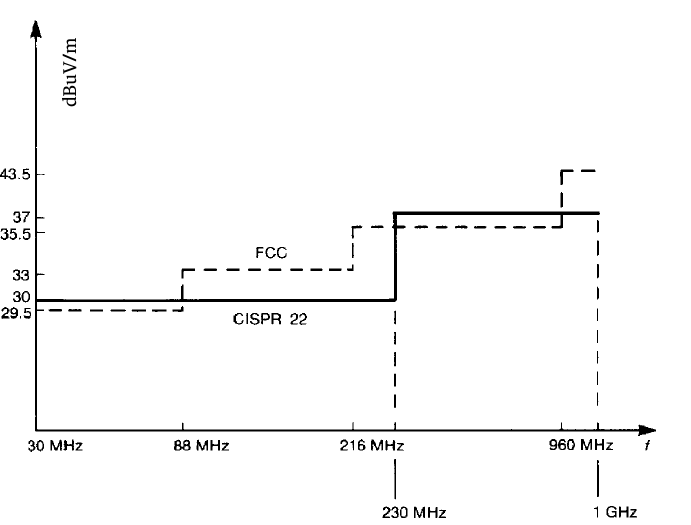
\includegraphics[scale=0.45]{./img/FCC_CISPR_10m_classB}}
	\subfloat[][Limites emissão irradiada - Classe A]{
		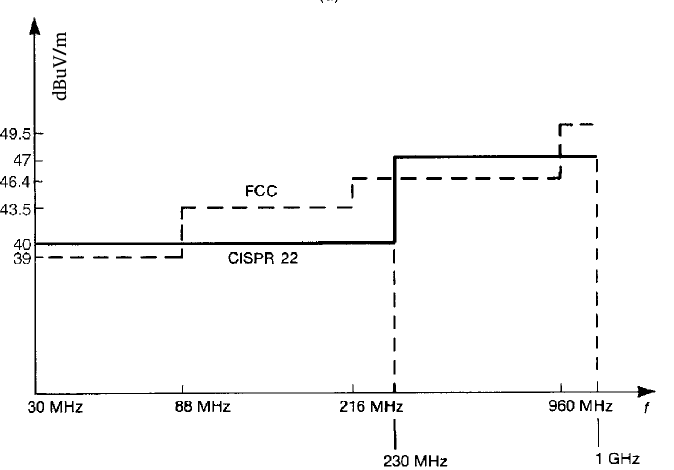
\includegraphics[scale=0.5]{./img/FCC_CISPR_10m_classA}}
    \fonte{Adaptado de~\citeonline[p.~55]{paul2006}}
\end{figure}

A maioria dos requisitos governamentais de EMC para mercados fora dos Estados Unidos Estados são estabelecidos pelo "\textit{Comité International Special des Perturbations Radioélectriques} - (CISPR), que é um comitê da International Electrotechnical Commission (IEC). Embora a CISPR escreva padrões, eles não são obrigatórios. No entanto, a maioria países internacionais adotam as recomendações da CISPR. O mais amplamente utilizado padrão é o CISPR 22, que estabelece limites para as emissões irradiadas e conduzidas de equipamento de tecnologia da informação, que inclui basicamente dispositivos digitais
no significado semelhante ao da FCC. Os limites são divididos em Classe A e Classe B, e seu significado é essencialmente o mesmo que as definições da FCC~\cite[p.~55]{paul2006}.

% Requisitos Funcionais (Susceptibilidades) 2.2(paul2006)
Como mencionado anteriormente, não é inteligente projetar um produto que realize alguma
função comercial sem que este não cumpra os requisitos regulamentares de EMC. Similarmente, também não é inteligente projetar um produto que atenda aos requisitos regulamentares de EMC estabelecidos pelas agências governamentais, mas não funcionar satisfatoriamente quando colocado perto de um transmissor de rádio FM ou de um radar de vigilância aeroportuária. Os consumidores não irão se satisfazer caso haja problemas causados por esses emissores no funcionamento dos dispositivos. Eles esperam que um produto que foi adquirido de boa fé funcione satisfatoriamente em qualquer instalação residencial, e o consumidor também não ficará satisfeito se houver um aviso que afirma “Cuidado, este computador não funcionará se sua casa estiver em um raio de 1 km de uma torre de transmissão FM"~\cite[p.~79]{paul2006}.. 

Igualmente embaraçoso seria se algum produto funcionar adequadamente, porém se o operador, através de um tapete de nylon em um escritório situado em um clima seco, toca o produto, causando uma descarga eletrostática que reinicializa a máquina. Por isso releva-se a importância do fabricante de impor determinados testes para além dos necessários por agências governamentais, a fim de garantir que o produto funcione adequadamente em uma ampla variedade de instalações de campo~\cite[p.~79]{paul2006}. 

\section{Análises de EMC em Placas de Circuito Impresso}
Os equipamentos eletrônicos são fabricados em 99,9\% dos casos utilizando uma placa de circuito impresso (PCI), sendo assim, é de extrema importância conhecer métodos e técnicas de análise de EMC em PCIs, para além disso, também conhecer soluções de leiaute e de fabricação destas placas, afim de minimizar o impacto e custos de correções destinadas a melhorias da compatibilidade eletromagnética.

% Como é feito as analises de EMC em Placas
As emissões eletromagnéticas de uma PCI são classificadas como emissões conduzidas e irradiadas ou emissões em modo comum e modo diferencial. As medidas das emissões conduzidas são realizadas com o uso de uma LISN, como visto anteriormente. Quanto as medições de emissões irradiadas, existem vários métodos de análises disponíveis~\apud[p.~12]{sivaraman2017}{hoolihan2017}, sendo que o método de maior interesse neste trabalho é o método de varredura de superfície.

Neste método as emissões irradiadas do \textit{Device Under Test} (Dispositivo sob teste - DUT) podem ser medidas por varredura com uma sonda acima do DUT. Na Figura~\ref{fig:scanning} podemos visualizar o esquema de um sistema de varredura automático de obtenção de medidas de emissões irradiadas. O resultado da medição do método de varredura de superfície fornece não apenas os campos eletromagnéticos do DUT, mas também a força relativa das fontes. além disso neste método pode ser usado uma variedade de sondas, como sondas elétricas, magnéticas e ópticas.

\begin{figure}[htb!]
	\centering 
	\caption{Sistema de Varredura - EMC}
	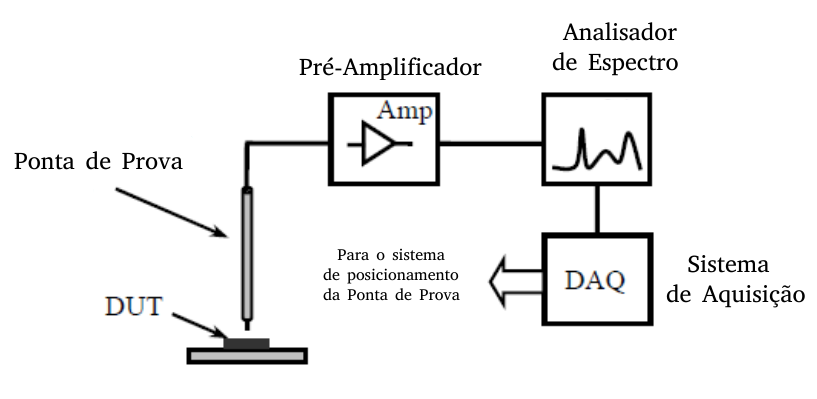
\includegraphics[scale=0.6]{./img/scanning_sistema}
	\fonte{Adaptado de~\citeonline[p.~13]{sivaraman2017}}
	%\legend{\hspace{-218pt}Fonte:~\citeonline[p.~8]{paul2006}}
	\label{fig:scanning}
\end{figure}

O método de varredura, utilizando pontas de provas para detecção de campo eletromagnético próximo é um método geral para identificar a fonte de EMI em circuitos eletrônicos. Vários métodos foram desenvolvidos por muitos autores para o cálculo do padrão de campo distante levando à identificação da fonte do campo. Entretanto, também é necessário conhecer os campos eletromagnéticos em suas características próximas~\apud[p.~17]{sivaraman2017}{gilabert2007}.

% EMC Conuduzida
% EMC Irradiada
% Problematização para detectar o foco do problema em EMC Irradiada

\section{Medidas de Campo Próximo}

As emissões eletromagnéticas irradiadas podem ser medidas em campo próximo ou distante. 

Para a qualificação junto as agencias reguladoras, as medições em campo distante são realizadas, como visto, em 3m e 10m, dependendo da agência. Existe ainda uma serie de procedimentos a serem seguidos, que não serão foco neste trabalho, apenas mencionará-se de forma sucinta que, basicamente, os campos elétricos irradiados para os testes comerciais (FCC e CISPR 22) devem ser medidas em um local de teste de área aberta (\textit{Open-Area Test Site} - OATS) ou em uma câmara semi-anecoica (\textit{Semi Anechoic Chamber} - SAC). Enquanto o OATS é o preferido, o SAC fornece
capacidade de medição em qualquer condição climática, bem como segurança. Uma câmara semi-anecoica é um local blindado com material absorvedor de radiofrequência nas laterais e no topo para evitar reflexões e simular o espaço livre, existem dois propósitos para a câmara semianecoica. O primeiro é evitar que as emissões eletromagnéticas de fora da sala contaminem o teste. A segunda é evitar reflexões nas paredes, de modo a simular o espaço livre, e esse recurso é fornecida pelo material do absorvedor de radiofrequência que reveste as paredes.

As medições realizadas em campo próximo têm como vantagens a precisão, confiabilidade, custo e faixa de aplicação. Em comparação com medições de campo distante, temos que o efeito de alguns fatores incertos, como clima, espalhamento, interferência eletromagnética tem menos influência nas medições de campo próximo porque a sonda e o equipamento sob teste (\textit{Device Under Test} - DUT) estão muito próximos uns dos outros e, portanto, fornecem uma medição mais precisa~\cite{sivaraman2017}.

% O que é Campo Proximo (Near-Field)
% Quais Campos próximos são de interesse aqui

\subsection{Campo Próximo e Campo Distante}
% Diferenças entra os campos próximos e distantes
Para compreendermos melhor as definições temos que o espaço ao redor de uma antena pode ser dividido em três regiões, campo próximo reativo, campo próximo radiativo e campo distante. 

O campo próximo reativo é aquela parte da região do campo próximo imediatamente ao redor
a antena, ou ponta de prova, onde que, para a maioria das antenas, o limite externo desta região é considerado como uma distância $R < 0.62 \sqrt(\frac{D^3}{\lambda})$~\cite[p.~34]{balanis2005}.

O campo próximo radiativo é definido como “aquela região do campo de uma antena entre a região reativa do campo próximo e a região do campo distante e em que a distribuição do campo angular depende da distribuição a partir da antena"~\cite[p.~34]{balanis2005}. Esta região também é conhecida com região de \textit{Fresnel}, fazendo uma analogia com a óptica, esta região é normalmente delimitada por $0.62 \sqrt(\frac{D^3}{\lambda}) < R < 2 \frac{D^2}{\lambda}$

A região de campo distante, ou região de \textit{Fraunhofer} é definida como aquela região do campo de uma antena onde a distribuição angular é independente da distância da antena. Se D é a dimensão global máxima do antena, a região do campo distante está a uma distância maior que  $R > 2 \frac{D^2}{\lambda}$~\cite[p.~16]{sivaraman2017}.

\begin{figure}[htb!]
	\centering 
	\caption{Campos Proximos e Distante}
	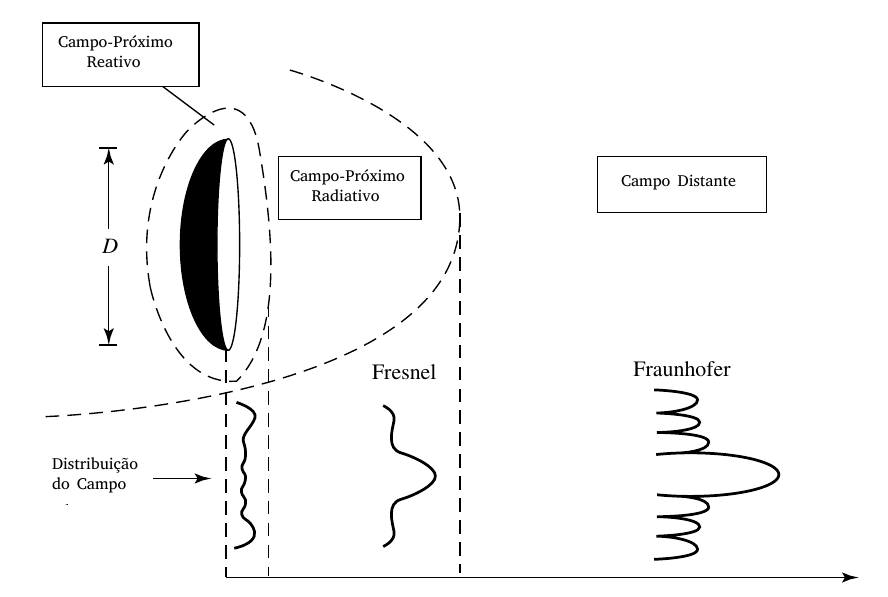
\includegraphics[scale=0.6]{./img/campos_balanis}
	\fonte{Adaptado de~\citeonline[p.~35]{balanis2005}}
	%\legend{\hspace{-218pt}Fonte:~\citeonline[p.~8]{paul2006}}
	\label{fig:regions_campos}
\end{figure}

Na figura~\ref{fig:regions_campos} há descrito as regiões que formam cada tipo de campo, é preciso destacar que as limitações destas regiões são válidas para a condição de $D >\lambda$, vemos também como se comporta a distribuição do campo em cada região.
%To be valid, D must also be large compared to the wavelength (D > λ).

%\subsection{Campo Magnético e Elétrico Próximo}
% Equacionamento Campo Mag e Ele proximos

\section{Pontas de Prova para Campo Próximo}
% Pontas de provas para Campos Proximos
As pontas de provas podem ser aplicadas de duas formas distintas na obtenção de medidas de campo próximo. A primeira configuração é com uma única sonda controlada por um sistema de posicionamento preciso. Na segunda, utiliza-se uma matriz planar de sondas afim de se obter várias medidas simultaneamente. Na figura~\ref{fig:medidas_sondas} visualizamos estas duas diferentes formas de medidas de campo próximo utilizando pontas de provas.

\begin{figure}[htb!]
	\centering 
	\caption{Tipos de medidas de campo próximo}
	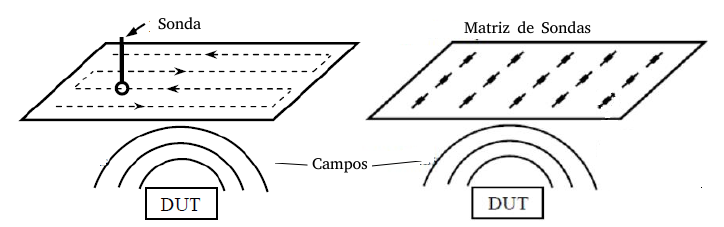
\includegraphics[scale=0.75]{./img/medidas_sondas}
	\fonte{Adaptado de~\citeonline[p.~21]{sivaraman2017}}
	%\legend{\hspace{-218pt}Fonte:~\citeonline[p.~8]{paul2006}}
	\label{fig:medidas_sondas}
\end{figure}

Segundo ~\citeonline[p.~21]{sivaraman2017} a aplicação mais utilizada é na forma de varredura, pois "A presença de um grande número de sondas induz distúrbios de primeira ordem no campo medido".

As pontas de prova de campo próximo (\textit{Near-Field Probe} - NFP) têm sido amplamente estudadas nos últimos anos devido à sua capacidade de quantificar a força do campo próximo (ótico, elétrico ou magnético) no espaço próximo ao sinal fonte. A maioria dos estudos sobre as NFP focou na melhoria da resolução espacial, largura de banda disponível, e suprimindo o campo acoplado em uma direção ortogonal ou campo adverso~\cite[p.~21]{sivaraman2017}. 

% Equacionamento

\subsection{Pontas de Prova Eletro-Ópticas}
% Caracteristicas das pontas eletro-opticas
Um tipo de NFP existente é a eletro-óptica, que consiste em uma sonda que pode ser utilizada para medidas de campos próximos elétricos e magnéticos, tendo como característica a conversão de um sinal eletro-magnético(obtido) para um sinal óptico(transmitido)~\cite[p.~22]{sivaraman2017}.

As ponta de provas ópticas são utilizadas no intuito de eliminar os distúrbios que as sondas metálicas convencionais (eletro-magnéticas) podem provocar no campo original, para isso, nas sondas ópticas há a presença de cristais opto-eletrônicos que convertem os campos medidos em sinais ópticos, não interagindo, de forma significativa, com o campo medido. \citeonline{arakawa2005} analisa a invasividade das sondas ópticas, de forma quantitativa, por simulação utilizando o método de diferenças finitas no domínio do tempo (FDTD). 

\subsection{Pontas de Prova Eletromagnéticas}
% Caracteristicas das pontas Eletromagnéticas
Outro tipo de NFP são as eletromagnéticas, que consistem, em espiras para o caso de detecção do campo magnético próximo, ou de um dipolo para o caso de detecção do campo elétrico próximo, e em ambos os casos, uma linha de transmissão para transportar o sinal induzido~\cite[p.~23]{sivaraman2017}. 

Um desenho comum para uma ponta de prova de campo elétrico consiste em um dipolo e uma linha de transmissão de fios paralelos. Pequenos dipolos são desejáveis ​​porque fornecem alta resolução espacial do campo, e porque permitem uma resposta independente de frequência. Um importante problema associado ao dipolo elétrico é a perturbação imposta ao dispositivo sob teste pela própria sonda~\cite[p.~23]{sivaraman2017}.

Neste trabalho, o foco são as NFP de campo magnético, que basicamente é composta por uma espira que opera de acordo com a lei de \textit{Faraday}

\begin{eqnarray}
\bigtriangledown \times E &=& -\frac{\partial B }{\partial t} \nonumber\\
V_{fem} &=& - \oint_C {E \cdot d\ell = - \frac{d}{{dt}}} \int_S {B_n dA} = -j\omega \mu H_nNA \label{FaradayLaw}
\end{eqnarray}

Onde, $\omega$ é a frequência angular, $\mu$ é a permeabilidade média no centro da espira, $H_n$ é a componente normal do campo magnético, $N$ é o numero de espiras e $A$ a área da espira. 

%Sabendo que: $\omega = 2 \pi f$, $\mu = 4 \pi 10^{-7}$ (no vácuo) e $H$ é a componente normal do campo magnético próximo, dado em $\frac{A}{m}$, temos que a Magnitude da tensão induzida pode ser determinada por:

%\begin{eqnarray}
%| V_{fem} | &=&  0.2 \pi f d^2 H \label{Vfem}
%\end{eqnarray}

A partir da equação~\ref{FaradayLaw} observa-se que a tensão induzida na sonda depende do tamanho da espira (sua área), dessa forma, a sensibilidade da sonda é diretamente proporcional ao tamanho da espira. Sabe-se também, que na sonda contêm não somente a corrente de circulação habitual, induzida pelo campo magnético, mas 
300também correntes que dependem do campo elétrico médio no plano do circuito. Erros grandes podem ser possíveis quando uma
espira é usada para medir campos magnéticos, a menos que seu diâmetro seja menor que $0.01 \lambda$~\cite[p.~25]{sivaraman2017} para não haver polarização do campo elétrico incidente.

Alguns estudos já foram realizados no que tange a fabricação de NFP de campo magnético próximo utilizando PCI. Existem métodos de fabricação de NFPs que vão desde a utilização de filmes finos depositados, tecnologia com semicondutor de metal-óxido complementar (\textit{Complementary Metal Oxide Semiconductor} - CMOS), NFPs integradas em circuitos integrados (CI), porém o foco deste trabalho está na obtenção de NFPs de baixo custo e de fácil fabricação, assim sendo os esforços estarão concentrados nas NFPs confeccionadas em PCIs. ~\citeonline{lin2009} traz o desenvolvimento de uma NFP em PCI com desempenho aprimorado. Na figura~\ref{fig:lin2009} visualizamos a topologia adotada, sendo fabricada sob um substrato de de fibra de vidro (FR4) que possui permissividade $\varepsilon = 4,4$ e espessura $ h = 0,8$mm. As dimensões utilizadas foram R = 4mm e d = 3.5mm e vemos o detalhe quanto ao filtro\textit{microstrip} (entalhes incorporados na linha de transmissão) que funcionam como um filtro para suprimir a auto-ressonância da espira, e, melhorar o desempenho da sonda em freqüências altas~\cite[p.~2]{lin2009}.

\begin{figure}[htb!]
	\centering 
	\caption{NFP com filtro \textit{microsrtip}}
	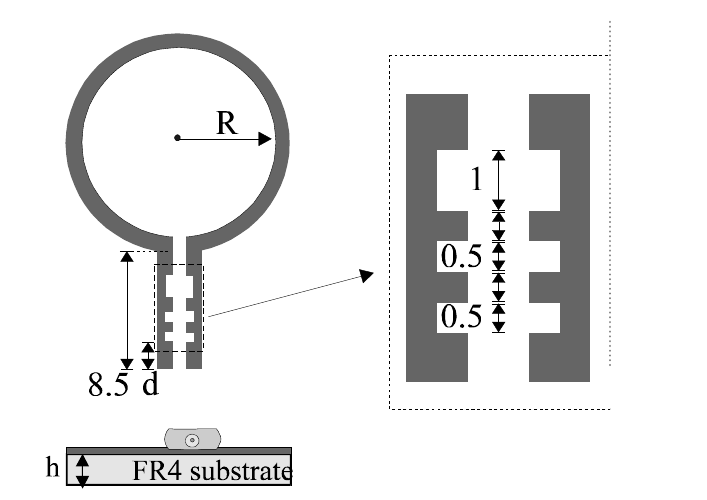
\includegraphics[scale=0.6]{./img/lin2009}
	\fonte{Adaptado de~\citeonline{lin2009}}
	%\legend{\hspace{-218pt}Fonte:~\citeonline[p.~8]{paul2006}}
	\label{fig:lin2009}
\end{figure}

~\citeonline{funato2006} desenvolveu duas topologias, a do tipo A com plano de terra e a do tipo B com uma linha recobrindo a trilha do sinal, na figura~\ref{fig:funato2006} pode-se observar a topologia desenvolvida, em ambas com a linha de transmissão tendo $50\Omega$ com $15$mm de comprimento, com uma espira quadrada contendo $1mm^2$ e confeccionada em FR4 (\textit{Flame Retardant 4} - Designação de classe para material laminado de epóxi reforçado com vidro utilizado em PCI).
\begin{figure}[htb!]
	\centering 
	\caption{NFP com Plano e Linha de Terra}
	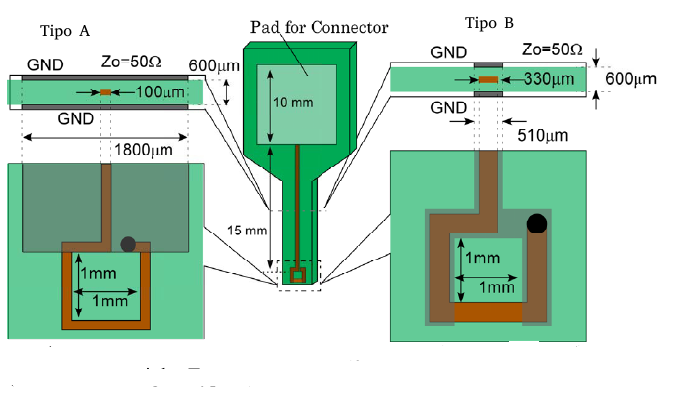
\includegraphics[scale=0.6]{./img/funato2006}
	\fonte{Adaptado de~\citeonline{funato2006}}
	%\legend{\hspace{-218pt}Fonte:~\citeonline[p.~8]{paul2006}}
	\label{fig:funato2006}
\end{figure}

